\documentclass[12pt,a4paper]{article}
\usepackage[utf8]{inputenc}
\usepackage[T1]{fontenc}
\usepackage{geometry}
\usepackage{graphicx}
\usepackage{booktabs}
\usepackage{array}
\usepackage{multirow}
\usepackage{amsmath}
\usepackage{lastpage}
\usepackage{fancyhdr}
\usepackage{titlesec}
\usepackage{xcolor}
\usepackage{hyperref}
\usepackage{capt-of}

\geometry{margin=1in}
\pagestyle{fancy}
\fancyhf{}
\rhead{\small NAPH 10th Annual Report Analysis}
\lhead{\small August 10, 2026}
\rfoot{\thepage/\pageref{LastPage}}

\hypersetup{
    colorlinks=true,
    linkcolor=blue!60!black,
    citecolor=blue!60!black,
    urlcolor=blue!60!black
}

\titleformat{\section}{\large\bfseries}{\thesection}{1em}{}
\titleformat{\subsection}{\normalsize\bfseries}{\thesubsection}{1em}{}

\begin{document}

\begin{titlepage}
\centering
\vspace*{2cm}
{\Huge\bfseries National Audit of Pulmonary Hypertension\\[0.5cm]
10th Annual Report — Data Analysis\par}
\vspace{1cm}
{\Large Comprehensive Analysis of Clinical Standards,\par
Patient Outcomes, and Centre Performance\par}
\vspace{2cm}
{\large\textbf{Report Date:} August 10, 2026\par}
\vspace{1cm}
{\small Based on data from the NAPH 10th Annual Report (October 2019)\par
and Supplementary Survival Analysis\par}
\vfill
\end{titlepage}

\tableofcontents
\newpage

\section{Overview: What Matters Most}

The National Audit of Pulmonary Hypertension (NAPH) 10th Annual Report evaluates the quality of care across eight specialist PH centres in Great Britain. This analysis examines 13 national standards, survival outcomes for over 23,000 patients in the longitudinal cohort (referred since April 2009), and centre-level performance patterns. The key findings are:

\begin{enumerate}
    \item \textbf{High overall compliance}: 11 of 13 national standards were met at the national level in 2018-19, demonstrating strong performance in diagnostic recording, catheterization rates, drug therapy appropriateness, and quality of life monitoring.
    
    \item \textbf{PEA waiting times remain a critical gap}: National Standard 13 (pulmonary endarterectomy within 4 months) was met by only 11\% nationally -- far below the 90\% target. Even among referral centres, results ranged from 0\% to 23\%, reflecting systemic capacity constraints at the single national PEA centre (Royal Papworth).
    
    \item \textbf{Significant mortality disparities exist}: At 5 years post-diagnosis, IPAH patients without comorbidities had survival rates ranging from 80\% (youngest females, age 18-41) down to 25\% (patients with comorbidities). Males consistently showed worse outcomes than females across all stratifications.
    
    \item \textbf{Patient volumes continue to grow}: Managed patient numbers increased from 5,705 (2009-10) to 10,572 (2018-19) -- an 85\% increase over the decade. Sheffield managed the largest caseload (1,926 active patients), while Newcastle had the smallest (361).
    
    \item \textbf{NS4 progress is notable but uneven}: All centres achieved above-target performance for NS4 (seen/discharge within 30 days) in 2018-19 for the first time, up from 53\% nationally in 2016-17 to 63\%. However, centre-level performance ranged from 53\% (Royal Papworth) to 100\% (Great Ormond Street).
\end{enumerate}

\section{Data and Methodology}

\subsection{Source Documents}
This analysis draws upon:
\begin{itemize}
    \item \textbf{NAPH 10th Annual Report} (October 2019) -- the main audit report covering 13 national standards evaluated across 8 specialist PH centres
    \item \textbf{Supplementary Survival Analysis} -- detailed Kaplan-Meier survival curves stratified by sex, age at diagnosis, and WHO functional class for patients with idiopathic pulmonary arterial hypertension (IPAH)
    \item \textbf{Local Action Plans} from five PH centres (Sheffield, Royal Brompton, Newcastle, Imperial College, Golden Jubilee) -- documenting improvement commitments where standards were not met
\end{itemize}

\subsection{Key Patient Cohorts}
\begin{itemize}
    \item \textbf{Managed patients (2018-19)}: 10,572 -- any patient with a referral active during the year
    \item \textbf{Active patients (March 31, 2019)}: 8,351 -- patients with referrals still open on the census date
    \item \textbf{Longitudinal cohort}: 23,311 adult patients whose first referral was on or after April 1, 2009; used for survival analysis
    \item \textbf{Active drug therapies (March 31, 2019)}: 4,683 patients with at least one PH drug prescribed
\end{itemize}

\subsection{Standards Evaluated}
Thirteen professionally agreed standards (National Standards 1--13) were assessed, set by the Pulmonary Hypertension Outcomes Group (PHOG). Targets range from 50\% to 100\% depending on clinical appropriateness. Standards rated at national level alone cover participation, timely diagnosis, catheterization, functional class documentation, vasoreactivity studies, pre-treatment therapy timing, diagnosis recording, quality of life measurement, annual consultations, and PDE5 inhibitor use as first-line therapy. Centre-level reporting covers standards applicable to all adult centres.

\section{Clinical Standards Performance}

\subsection{Standards Over Time (2015-16 to 2018-19)}

Table~\ref{tab:standards_trend} summarises performance trends for each standard across four audit years.

\begin{table}[htbp]
\centering
\resizebox{\textwidth}{!}{
\begin{tabular}{lccccl}
\toprule
\textbf{Standard} & \textbf{Target} & \textbf{2015-16} & \textbf{2016-17} & \textbf{2017-18} & \textbf{2018-19} & \textbf{Trend} \\
\midrule
NS3 Timely Diagnosis & 95\% & 96\% & 98\% & 98\% & \textbf{99\%} & Up ▲ \\
NS4 Seen Within 30d & 50\% & 47\% & 53\% & 60\% & \textbf{63\%} & Up ▲ \\
NS5 Pre-tx Catheterization & 95\% & 91\% & 96\% & 96\% & \textbf{97\%} & Static \\
NS6 Functional Class Recorded & 90\% & 80\% & 85\% & 98\% & \textbf{97\%} & Static \\
NS8 Drug Therapy $<$12wks & 80\% & 76\% & 82\% & 81\% & \textbf{81\%} & Static \\
NS9 Diagnosis Recorded & 99\% & 100\% & 100\% & 100\% & \textbf{100\%} & Static \\
NS10 PDE5 Inhibitor First-line & 80\% & 90\% & 92\% & 93\% & \textbf{91\%} & Static \\
NS11 Quality of Life Recorded & 90\% & 78\% & 89\% & 96\% & \textbf{96\%} & Static \\
NS12 Annual Consultation & 90\% & 96\% & 96\% & 96\% & \textbf{96\%} & Static \\
NS13 PEA Wait $<$4mo & 90\% & 14\% & 13\% & 18\% & \textbf{11\%} & Static --- \\
\bottomrule
\end{tabular}
}
\caption{National Standards performance trends. Bold values indicate 2018-19 figures. NS7 (Vasoreactivity Study) is new in 2018-19 at 57\% against an 80\% target.}
\label{tab:standards_trend}
\end{table}

Three standards showed statistically significant upward trends: NS3 (timely diagnosis, reaching 99\%), NS4 (seen within 30 days, rising from 47\% to 63\%), and NS5 (pre-treatment cardiac catheterisation, stabilising at 97\%). Standards 6 through 12 showed largely stable trajectories, having reached plateau levels in earlier years. Two standards fell far below their targets: notably NS13 (PEA waiting times) at just 11\% against a 90\% target.

\begin{figure}[htbp]
\centering
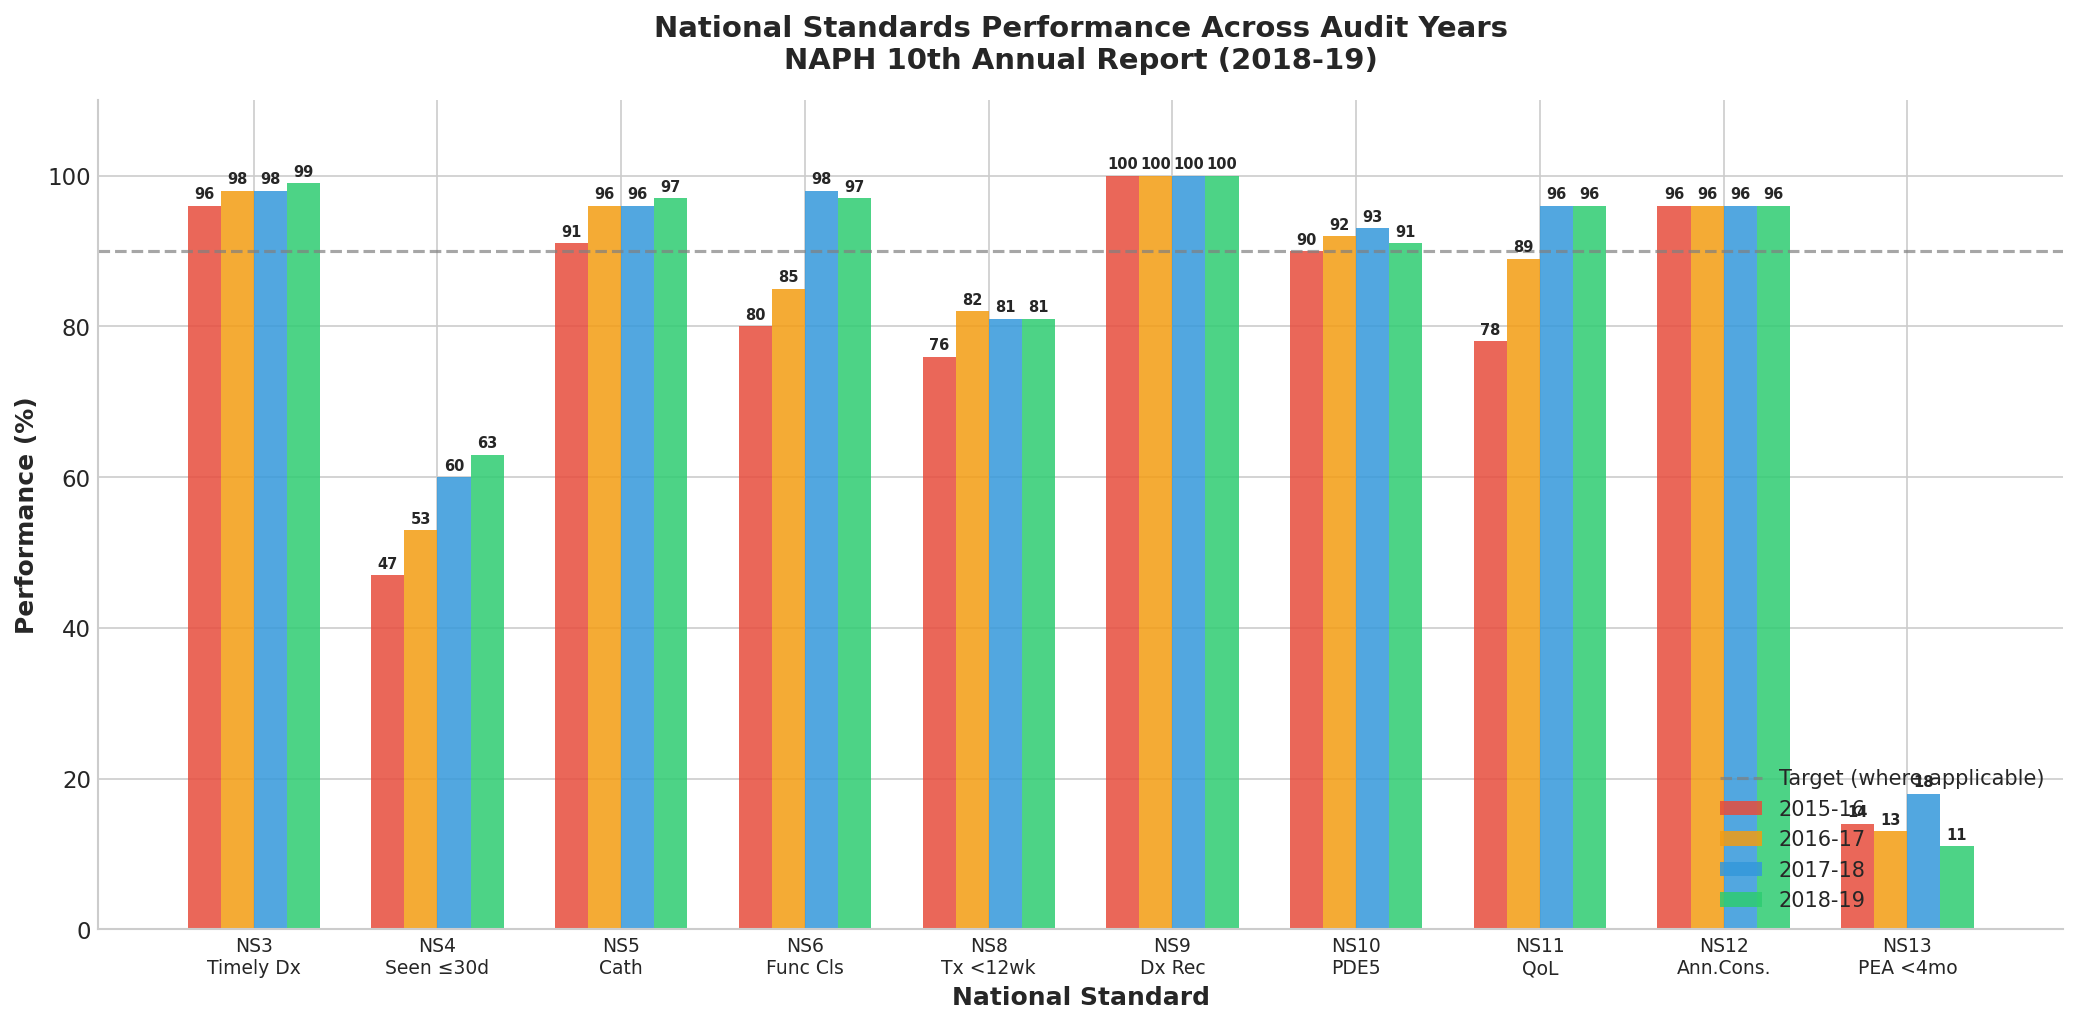
\includegraphics[width=\textwidth]{chart1_standards_performance.png}
\caption{National Standards performance across audit years (2015-16 to 2018-19). Note the dramatic gap between NS13 (PEA wait times) and all other standards.}
\label{fig:standards_over_time}
\end{figure}

\subsection{Centre-Level Performance Matrix (2018-19)}

Figure~\ref{fig:heatmap} presents a heatmap of centre-by-standard performance. Key observations include:

\begin{itemize}
    \item \textbf{No centre meets every standard}: Every PH centre misses at least one standard, confirming that systemic improvement opportunities persist even at high-performing centres.
    \item \textbf{Newcastle achieves excellence}: Newcastle is one of only two centres achieving 100\% on both NS3 (timely diagnosis) and NS9 (diagnosis recorded), alongside Sheffield (which scores 100\% on both). 
    \item \textbf{NS4 variability is large}: Performance on seen within 30 days ranges from 53\% (Royal Papworth) to 100\% (Great Ormond Street), highlighting process variation in triage and first appointment scheduling.
    \item \textbf{NS13 universally underperforming}: Only 1 of 7 adult centres (Golden Jubilee and Royal Papworth, both at 23\%) comes close to any meaningful proportion, reflecting the bottleneck at the single national PEA facility at Royal Papworth.
\end{itemize}

\begin{figure}[htbp]
\centering

\includegraphics[width=\textwidth]{chart7_standards_heatmap.png}
\caption{Performance matrix: National Standards by PH centre (2018-19). Green indicates meeting or exceeding the target; yellow indicates moderate performance; red indicates significant shortfall.}
\label{fig:heatmap}
\end{figure}

\subsection{NS4 Progression: A Success Story Worth Studying}

National Standard 4 (new patients seen or discharged within 30 days) shows marked improvement across all centres. Figure~\ref{fig:ns4_progression} illustrates this progression from 2015-16 to 2017-18.

\begin{figure}[htbp]
\centering
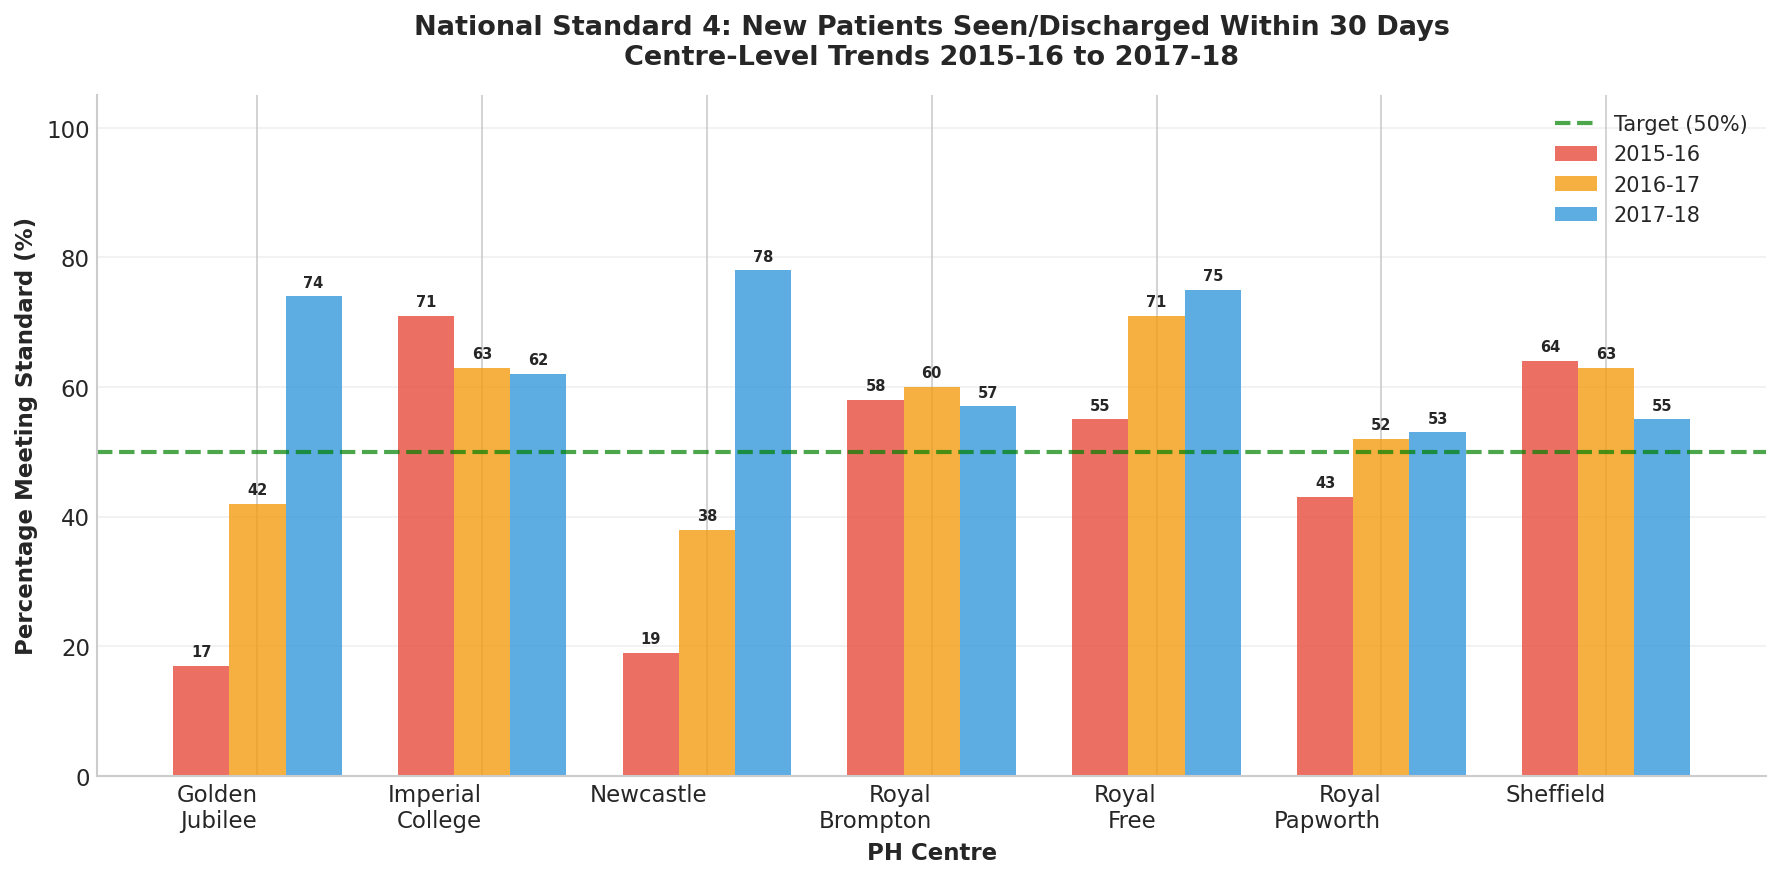
\includegraphics[width=\textwidth]{chart11_ns4_progression.png}
\caption{NS4 performance at centre level from 2015-16 to 2017-18. All centres crossed the 50\% target by 2017-18, with Newcastle showing the steepest improvement trajectory.}
\label{fig:ns4_progression}
\end{figure}

Notable examples: Newcastle improved from 19\% (2015-16) to 78\% (2017-18); Golden Jubilee rose from 17\% to 74\%. The report attributes these gains to additional appointment slots and dedicated new-patient pathways. Royal Brompton credits bi-monthly data review cycles and continuous error-flagging by the data entry manager. These practices warrant broader dissemination.

\section{Patient Volume Trends}

\subsection{National Growth Trajectory}

The number of managed patients has grown steadily over the 10-year period, increasing from 5,705 in 2009-10 to 10,572 in 2018-19 -- a near doubling (85\% increase). PAH/CTEPH-specific managed patients grew from 3,280 to 6,069 (85\%). Active patients (open referrals on March 31) expanded from 4,341 to 8,351 over a parallel period.

\begin{figure}[htbp]
\centering
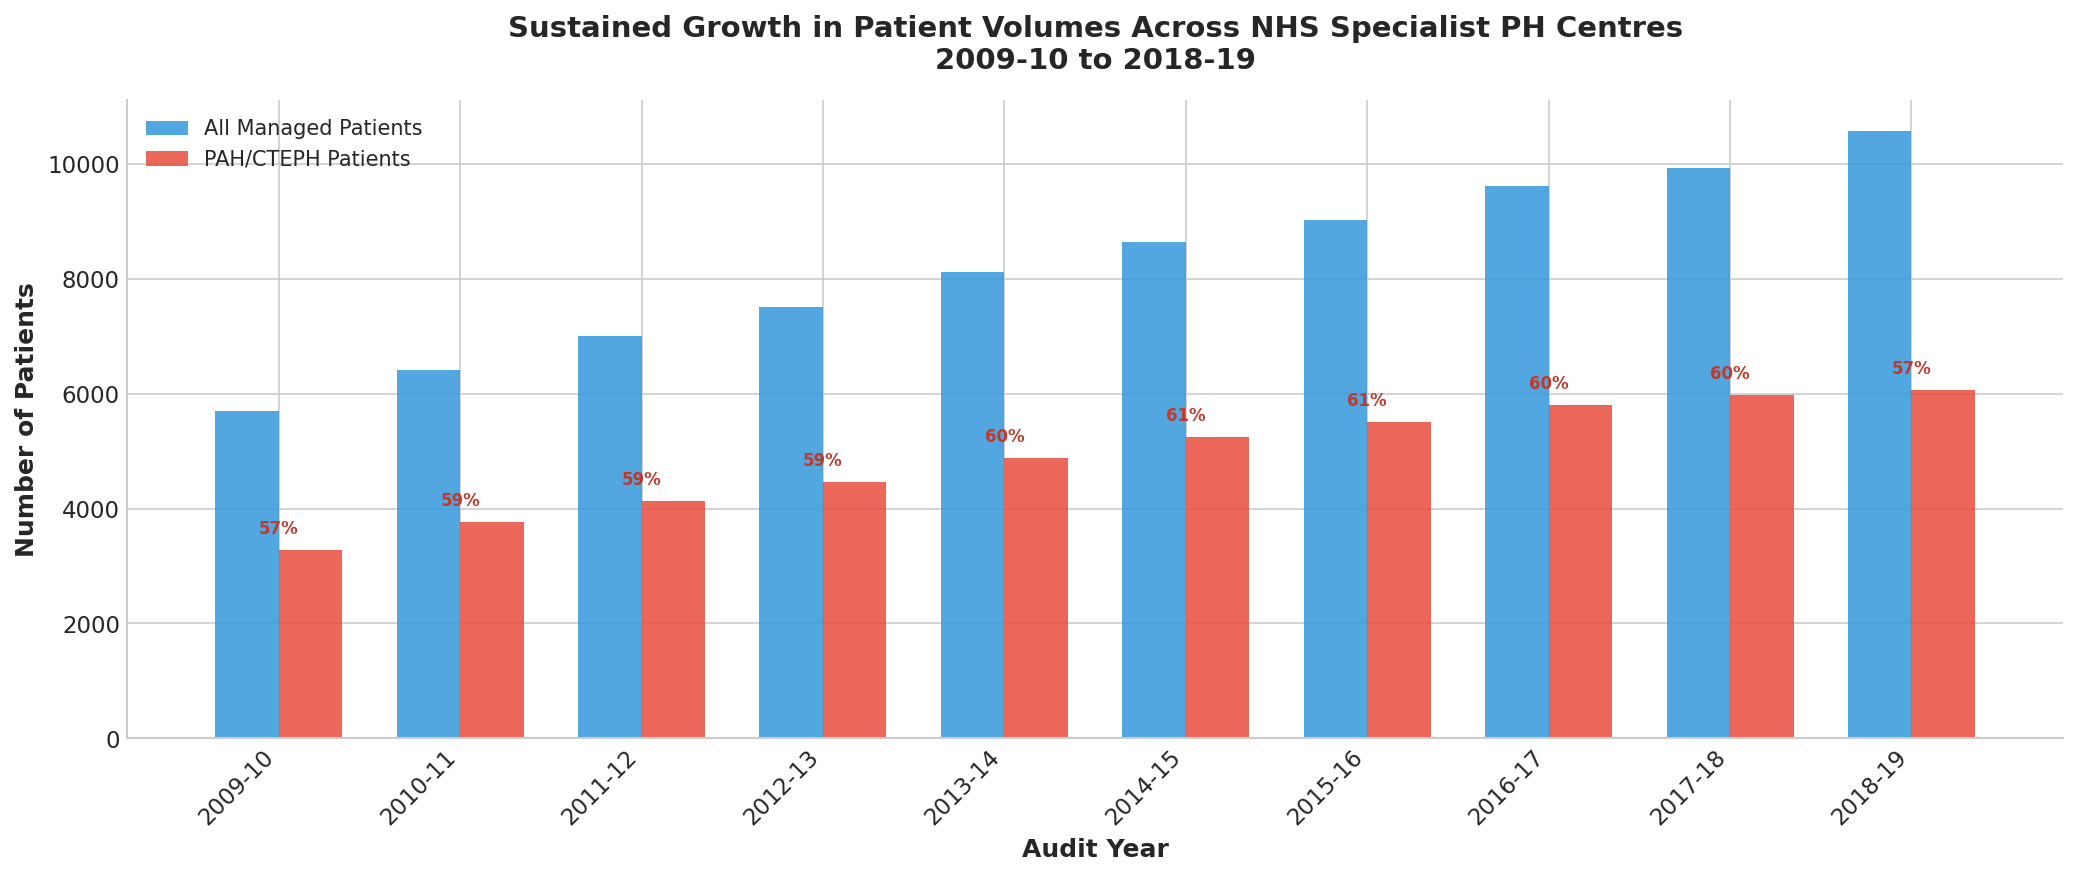
\includegraphics[width=\textwidth]{chart2_patient_volume_growth.png}
\caption{Sustained growth in total managed patients and PAH/CTEPH-specific patients across NHS specialist PH centres.}
\label{fig:volumes}
\end{figure}

This persistent expansion, noted in the foreword as ``unusually after 10 years it shows no signs of levelling off,'' has important implications for service planning, workforce allocation, and infrastructure needs.

\subsection{Centre-Level Caseloads (2018-19)}

\begin{figure}[htbp]
\centering
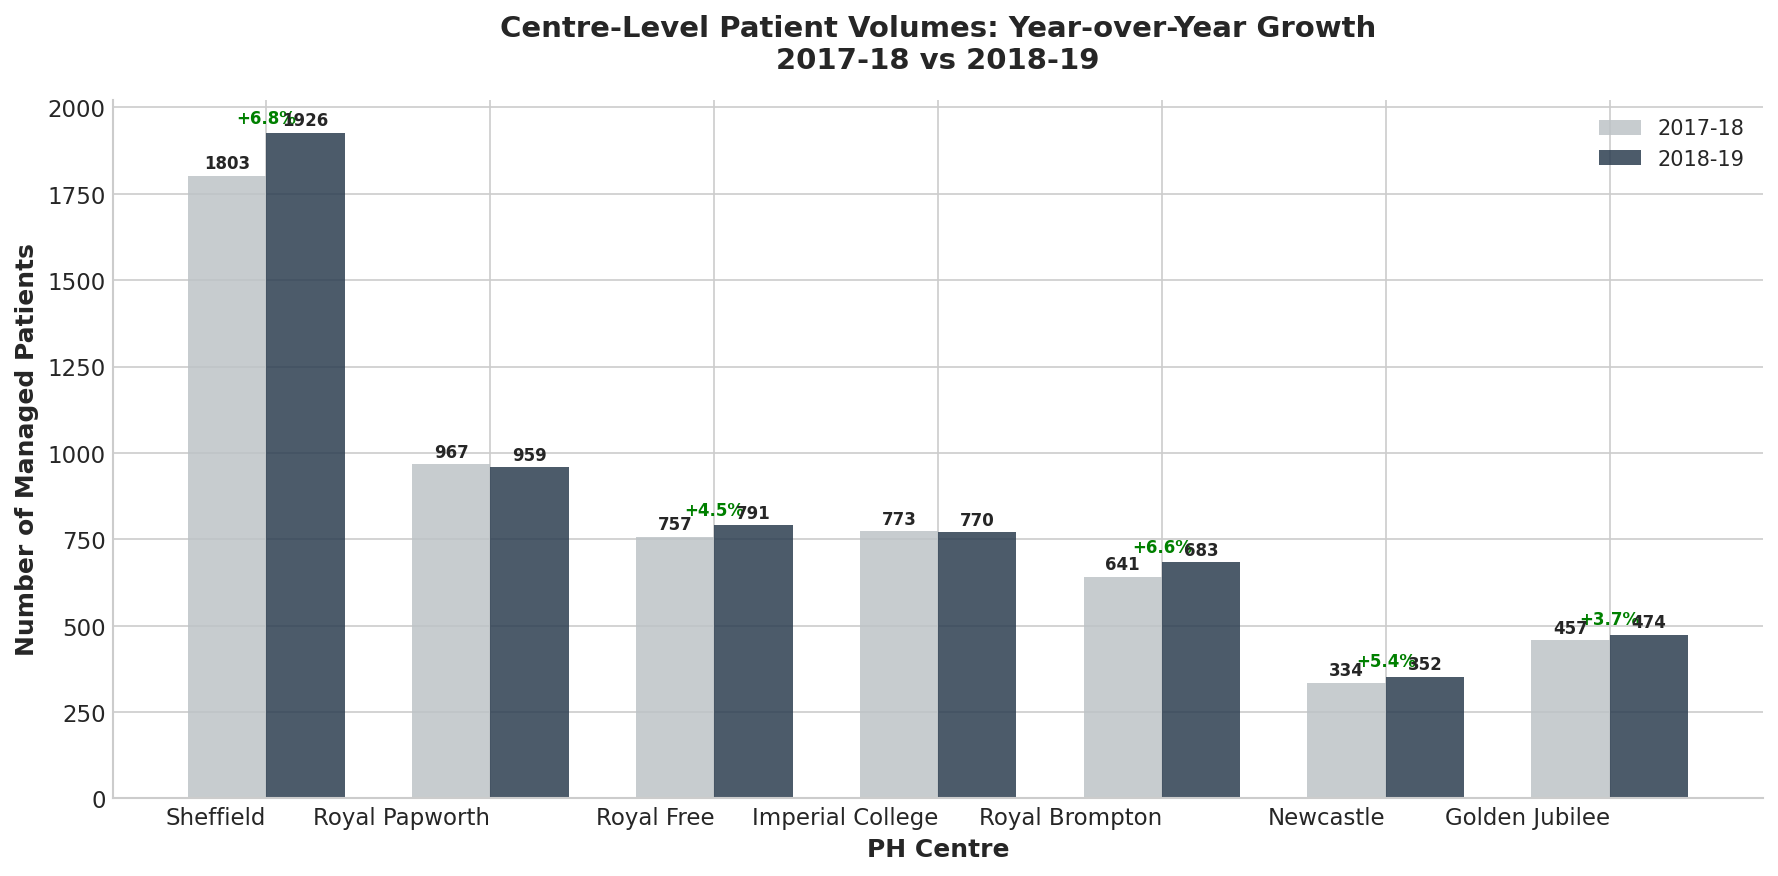
\includegraphics[width=\textwidth]{chart3_centre_volumes.png}
\caption{Centre-level patient volumes for 2017-18 and 2018-19. Sheffield manages the largest caseload by a substantial margin (nearly double Royal Papworth).}
\label{fig:centre_vol}
\end{figure}

Sheffield remains by far the largest centre (1,926 active patients in 2018-19), managing more than all other six adult centres combined would suggest a need for appropriately scaled staffing and facilities. Newcastle (361 active patients) operates at the lower bound of the national volume threshold of 300 PAH/CTEPH patients per annum -- although it comfortably exceeded this in managed volume (352).

All seven adult centres met Standard 2 (sufficient patient volume) in 2018-19, indicating that centre consolidation strategies from the early years of the audit have been successful.

\subsection{Diagnosis and Disease Distribution}

Among the 8,351 active patients in 2018-19:
\begin{itemize}
    \item \textbf{PAH}: 43\% (3,592 patients)
    \item \textbf{CTEPH}: 23\% (1,921 patients; of whom ~52\% operated, ~48\% not yet operated)
    \item \textbf{Left heart disease}: 5\%
    \item \textbf{Lung disease}: 4\%
    \item \textbf{Not pulmonary hypertension}: 16\% (suggests referral filtering opportunities)
    \item \textbf{Other/mixed categories}: remainder
\end{itemize}

Within PAH subtypes, idiopathic PAH (IPAH) accounts for 30\% of diagnoses, with connective tissue disease-associated PAH (CTD-APAH) representing 22\%. Scleroderma-related PAH constitutes 15\% nationally. Centre-level variation is striking: Sheffield reports 39\% IPAH versus Royal Brompton's 16\%; conversely, Royal Papworth reports 49\% CTD-APAH compared to 2\% at Newcastle.

\begin{figure}[htbp]
\centering

\includegraphics[width=\textwidth]{chart10_patient_characteristics.png}
\caption{Diagnosis type distribution among all active patients (left), and PAH subtype distribution among patients with a PAH diagnosis (right), Great Britain 2018-19.}
\label{fig:characteristics}
\end{figure}

\section{Drug Treatment Patterns}

\subsection{Treatment Evolution (2010--2019)}

Figure~\ref{fig:drug_trends} illustrates how therapeutic regimens have evolved across the decade. Three broad patterns emerge:

\begin{enumerate}
    \item \textbf{Sildenafil dominance}: Remains the most widely prescribed monotherapy throughout the decade, reaching 3,356 patients in 2018-19. Its share has remained relatively flat since 2015.
    \item \textbf{Macitentan emergence}: Started in 2015 (296 patients) and grew rapidly to become the second-largest agent by 2019 (1,139 patients), displacing older endothelin receptor antagonists.
    \item \textbf{Bosentan decline}: Fell from 1,141 patients (2012-13 peak) to 597 (2018-19), roughly halving as newer agents replaced it.
\end{enumerate}

Tadalafil also shows strong growth (from 3 patients in 2010 to 709 in 2019), reflecting the shift toward once-daily phosphodiesterase-5 inhibitors. Combined therapies (dual and triple) are increasingly common, consistent with global guideline recommendations to escalate treatment intensively.

\begin{figure}[htbp]
\centering
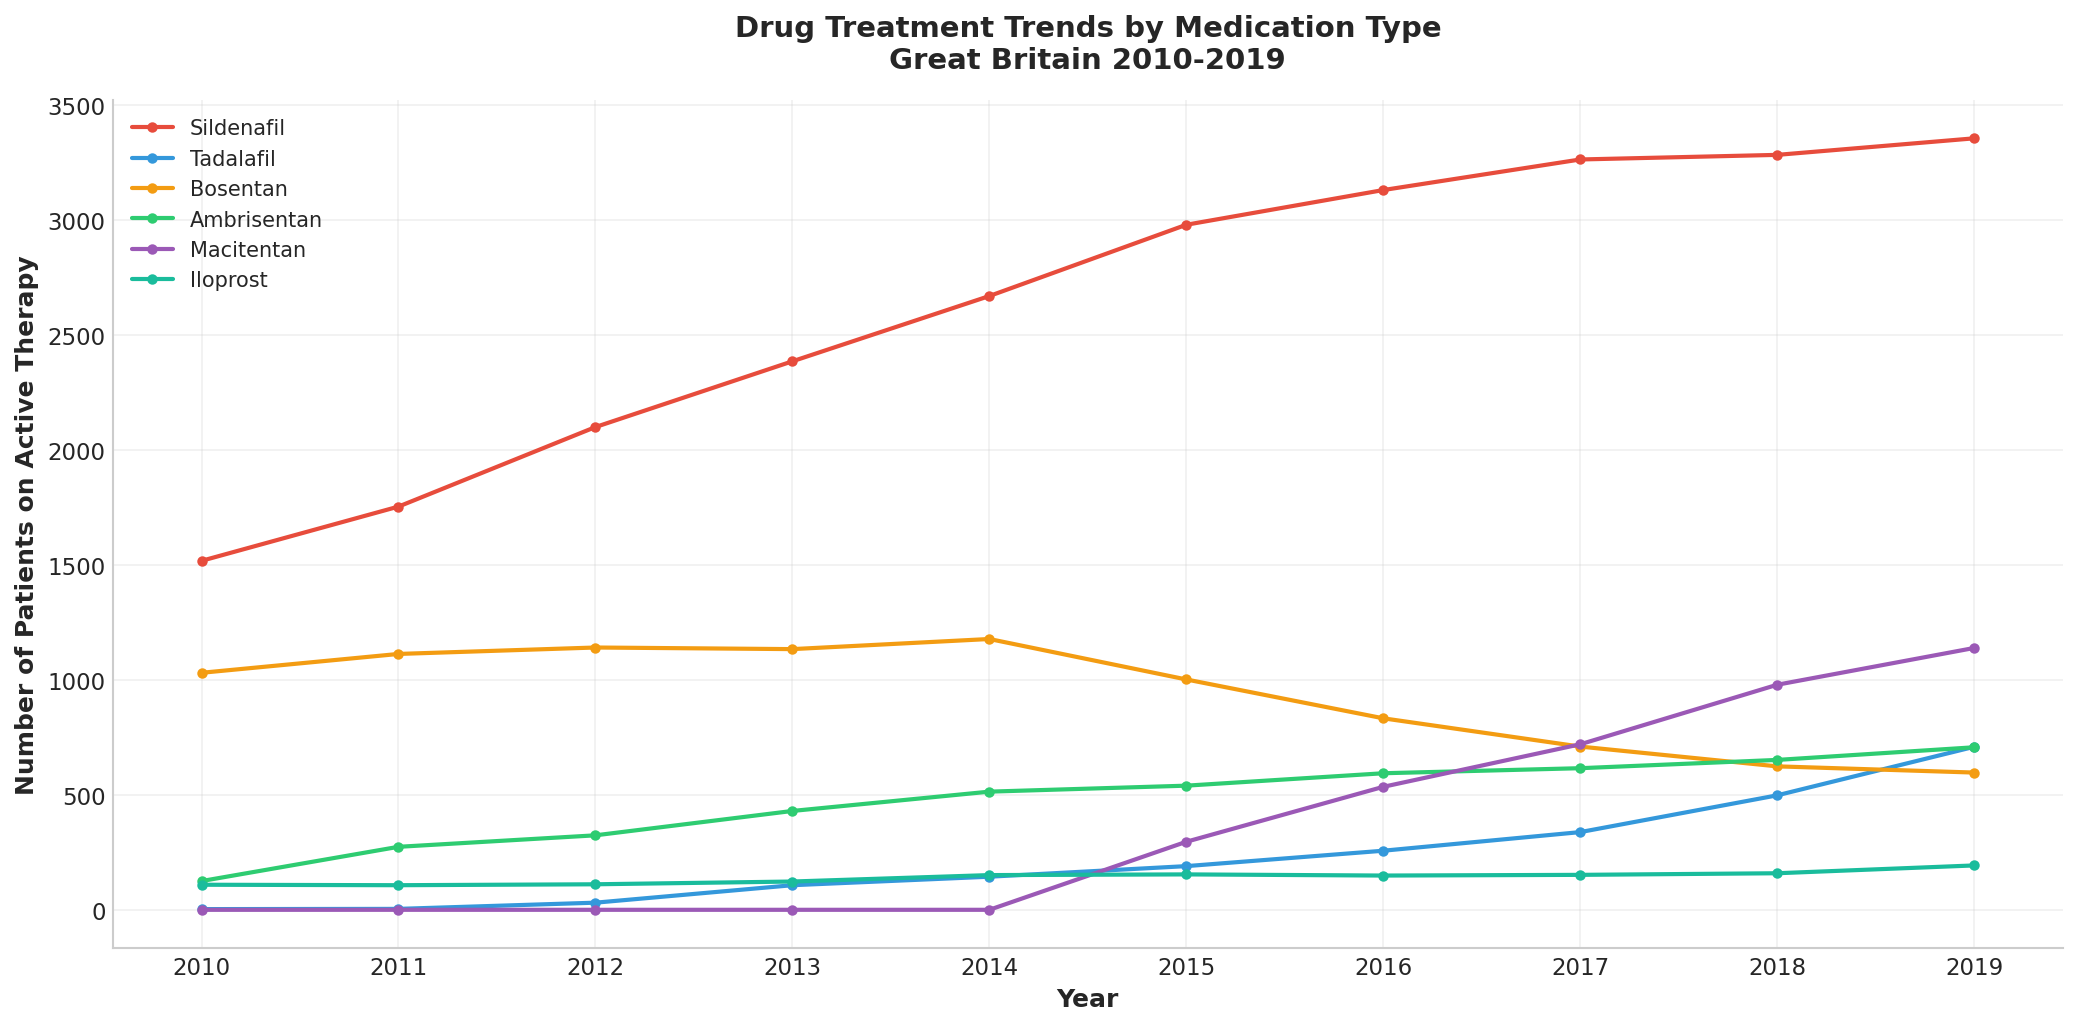
\includegraphics[width=\textwidth]{chart9_drug_trends.png}
\caption{Drug treatment adoption trends from 2010 to 2019, showing the transition from sildenafil-based regimens towards macitentan and tadalafil-based combinations.}
\label{fig:drug_trends}
\end{figure}

\subsection{Combination Therapy by Sex and Comorbidity Status}

Patients with IPAH without comorbidities are more likely to receive combination therapy (72\% dual+triple) compared to those with comorbidities (42\% dual+triple), suggesting either greater tolerability and willingness to escalate in younger, fitter patients or possibly undertreatment of the comorbidity group. Females with IPAH without comorbidities receive dual therapy more often (52\%) than males (49\%). Triple or greater therapy is rare outside the non-comorbidity group (9--12\%).

\begin{figure}[htbp]
\centering
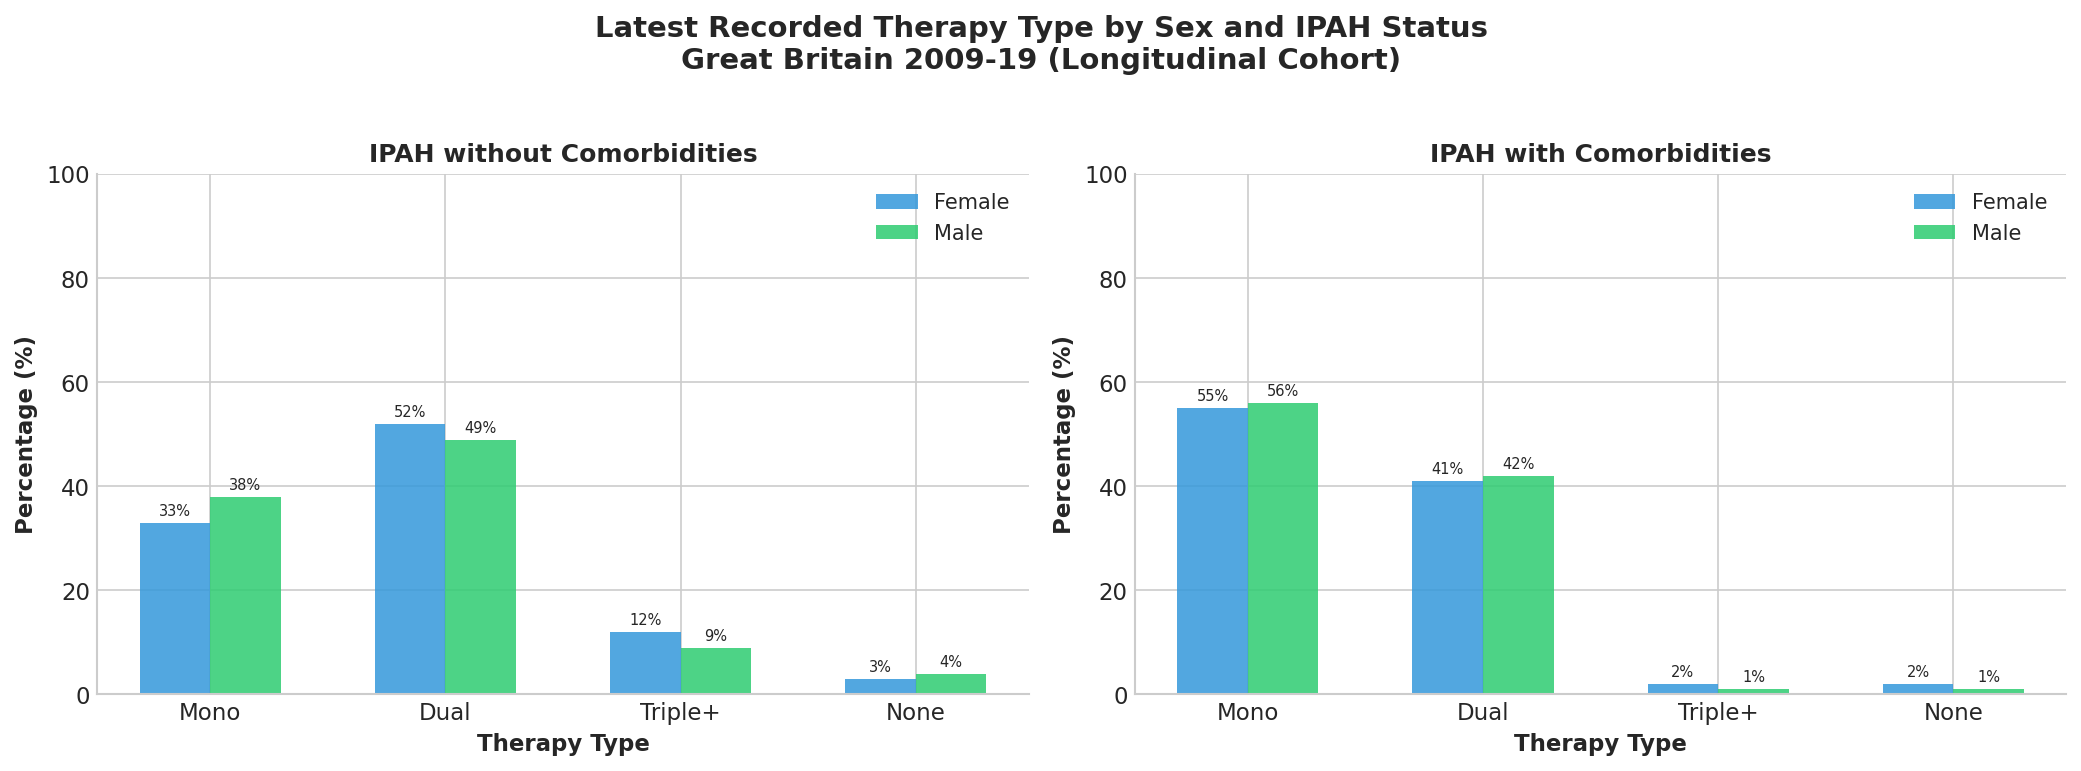
\includegraphics[width=\textwidth]{chart8_therapy_types.png}
\caption{Distribution of therapy intensity (monotherapy, dual, triple+, none) by sex and comorbidity status, derived from the latest recorded therapy date in the longitudinal cohort.}
\label{fig:therapy}
\end{figure}

\section{Survival Analysis}

Survival analysis is based on the longitudinal cohort of adult patients referred since April 2009, tracking deaths via direct submission by PH centres supplemented by Office for National Statistics (ONS) linkage. Scottish patients (Golden Jubilee) cannot be traced via ONS due to pseudonymisation and are therefore excluded from lung disease left-heart disease survival curves. Curves cease when fewer than 50 patients remain in the risk set.

\subsection{Overall Survival}

For the entire cohort, cumulative survival drops from 100\% at diagnosis to approximately 85\% at 1 year, 75\% at 2 years, 60\% at 3 years, 50\% at 4 years, and 45\% at 5 years. Half-lives vary substantially by patient characteristics described below.

\subsection{Survival by Sex}

Figure~\ref{fig:survival_sex} reveals striking survival differences by sex:

\begin{itemize}
    \item \textbf{Females with IPAH without comorbidities}: Best outcomes; 75\% survive to 3 years, 60\% to 5 years, and 48\% to 8 years. Median survival exceeds 7 years and 77 days.
    \item \textbf{Males with IPAH without comorbidities}: Worse than females; only 60\% survive to 3 years and 36\% to 6 years. Median survival is 3 years and 279 days -- roughly half that of females.
    \item \textbf{Both sexes with comorbidities}: Poor prognoses; females reach only 45\% at 3 years and 40\% at 4 years. Males drop to 40\% by year 3. The median survival is 2 years and 244 days (females) to 2 years and 211 days (males).
\end{itemize}

\begin{figure}[htbp]
\centering
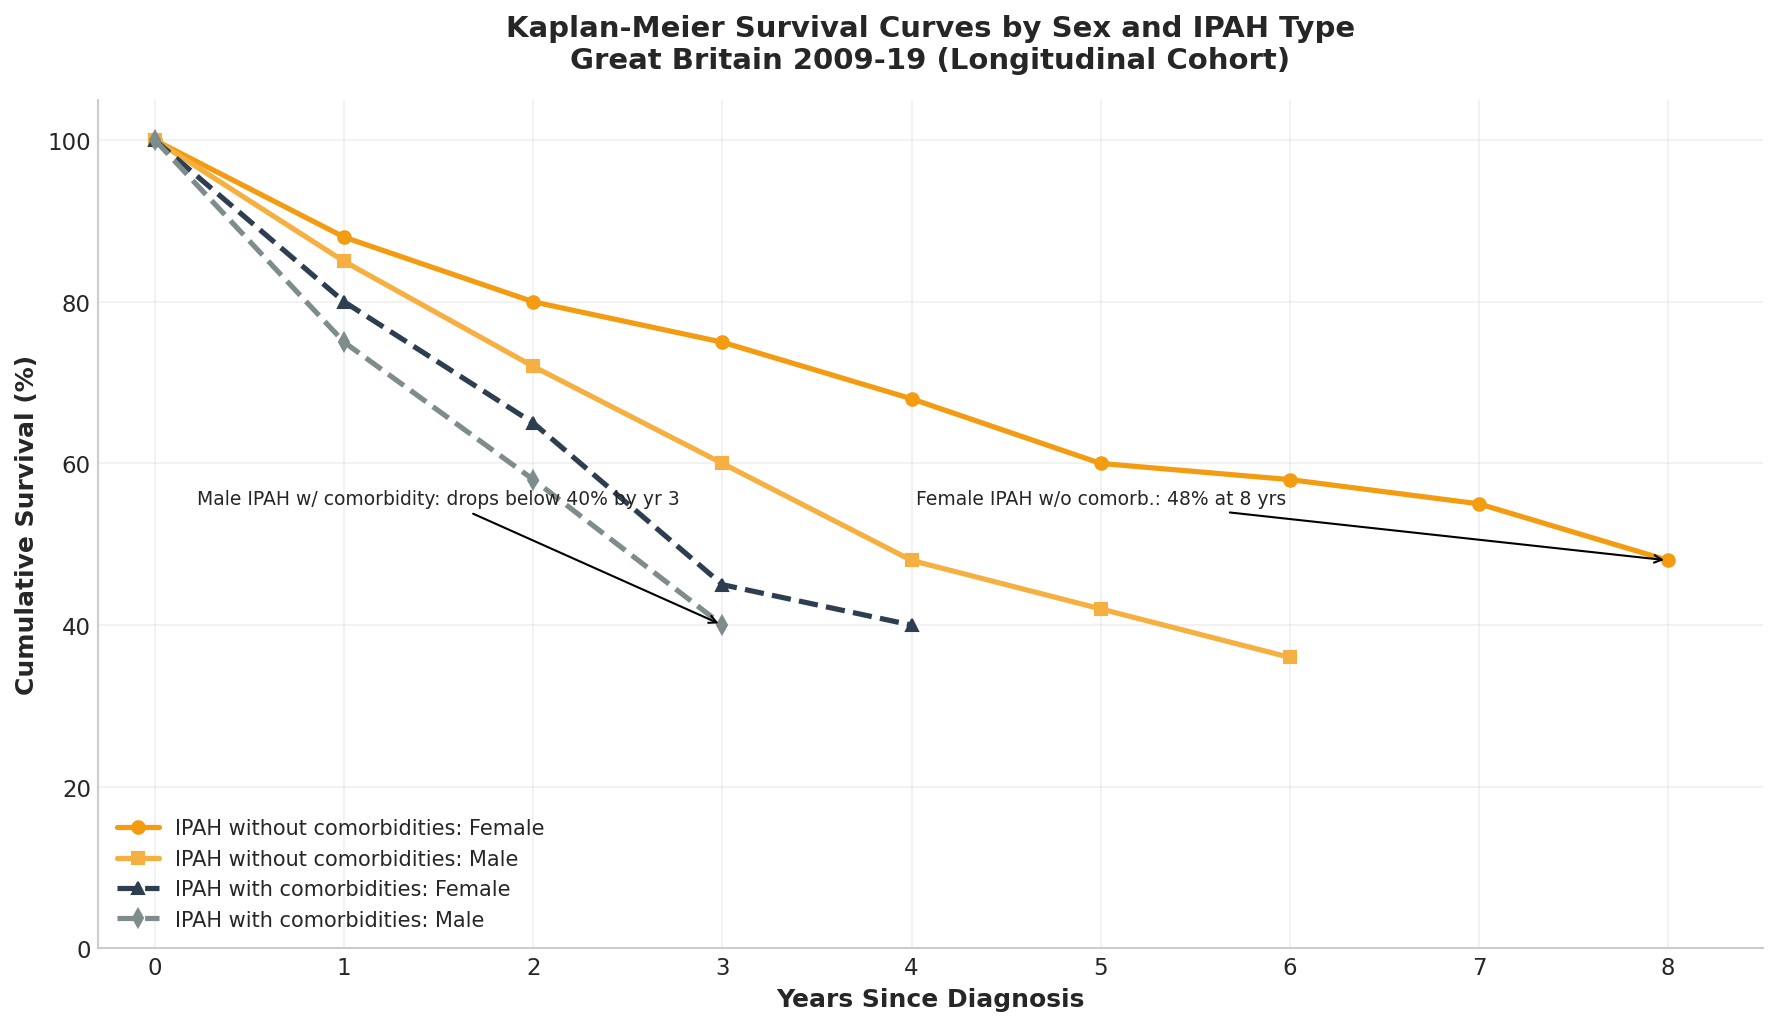
\includegraphics[width=\textwidth]{chart4_survival_by_sex.png}
\caption{Kaplan-Meier survival curves stratified by sex and IPAH type. The sex gap is pronounced in IPAH without comorbidities.}
\label{fig:survival_sex}
\end{figure}

\subsection{Survival by Age at Diagnosis}

Age is a powerful determinant of survival independent of comorbidity status (Figure~\ref{fig:survival_age}):

\begin{itemize}
    \item \textbf{Quintile 1 (age 18--41)}: Exceptional outcomes; 80\% survival persists at 5 years, and 78\% at 6 years. The median survival point had not been reached at 6 years and 218 days.
    \item \textbf{Quintile 2 (age 41--54)}: Strong outcomes; 75\% survival at 5 years, 70\% at 6 years.
    \item \textbf{Quintile 3 (age 54--66)}: Intermediate; 45\% at 5 years, median at 4 years and 127 days.
    \item \textbf{Quintile 5 (age 74--91)}: Poorest of the non-comorbidity groups; 30\% at 5 years, median at 2 years and 291 days.
    \item \textbf{IPAH with comorbidities}: Equivalent to or worse than Quintile 5 despite including younger patients; 25\% at 5 years, median at roughly 2 years and 218 days.
\end{itemize}

\begin{figure}[htbp]
\centering
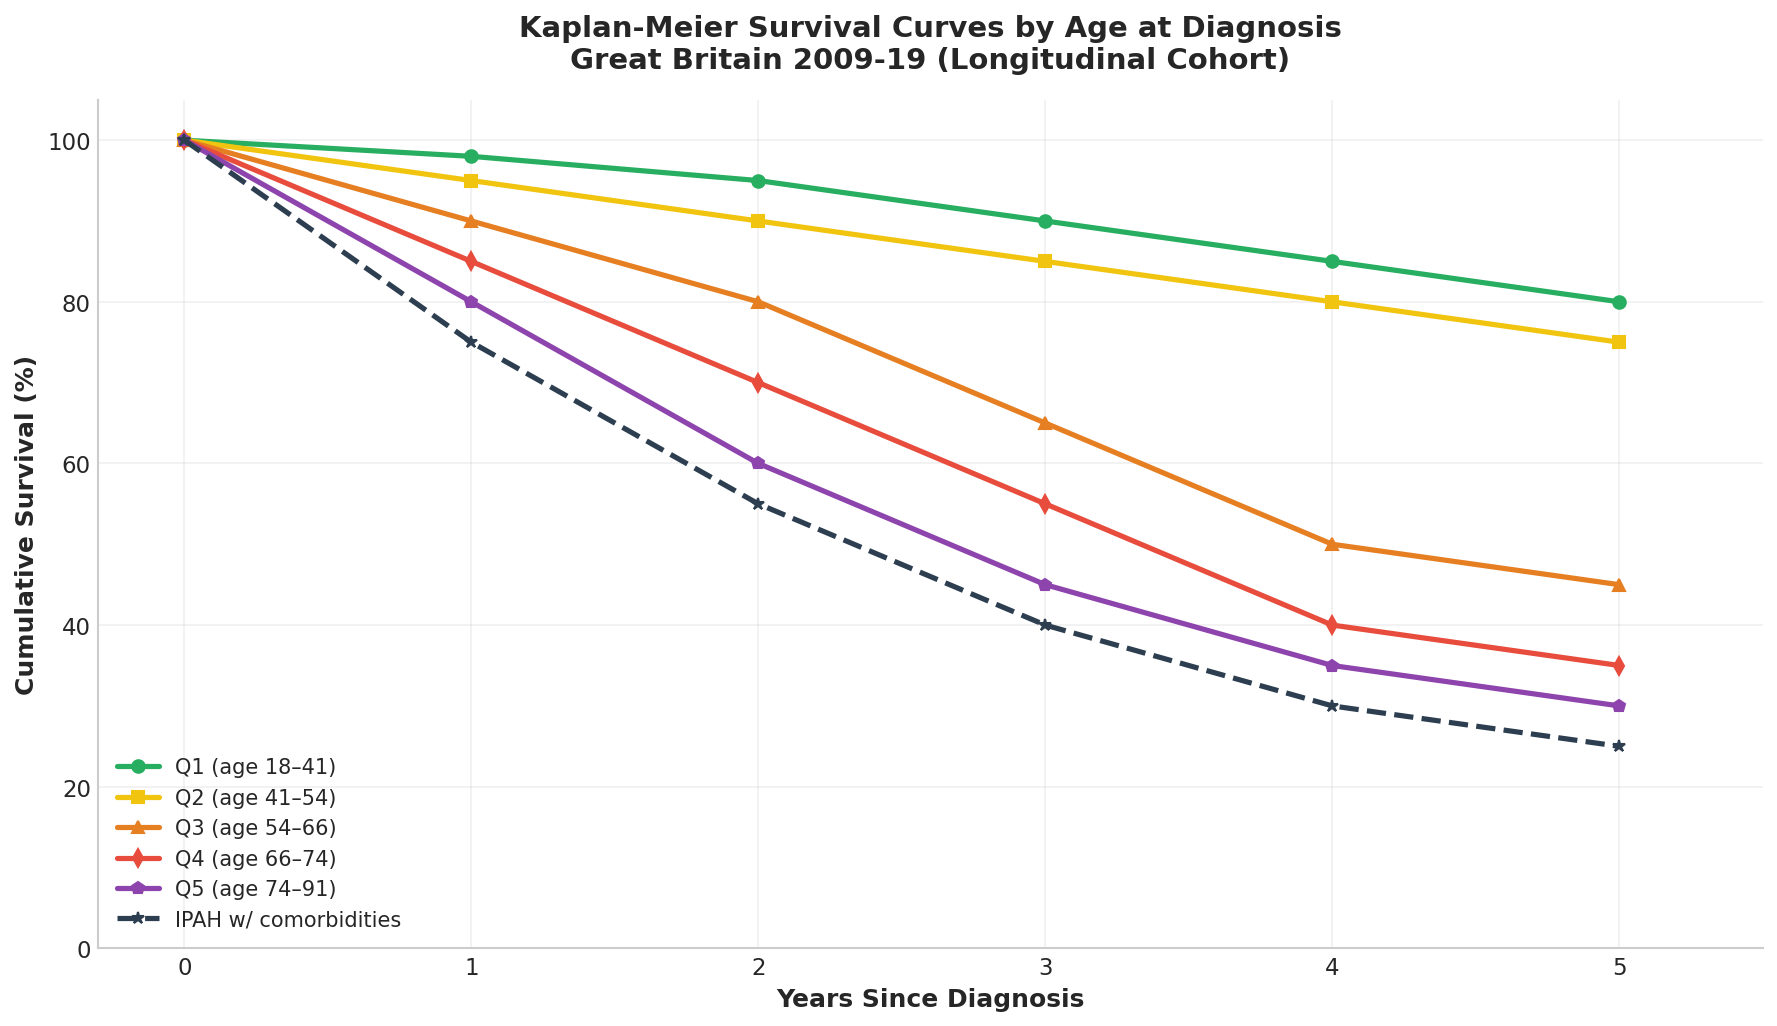
\includegraphics[width=\textwidth]{chart5_survival_by_age.png}
\caption{Kaplan-Meier survival curves stratified by age quintiles among IPAH patients without comorbidities, alongside the combined comorbidity group. Younger patients show markedly superior survival.}
\label{fig:survival_age}
\end{figure}

\subsection{Survival by WHO Functional Class}

WHO functional class at diagnosis powerfully predicts downstream outcomes (Figure~\ref{fig:survival_who}):

\begin{itemize}
    \item \textbf{WHO Class II (without comorbidities)}: 95\% survival at 1 year, 75\% at 4 years. Notably good prognostic profile.
    \item \textbf{WHO Class III (without comorbidities)}: 90\% at 1 year, declining to 43\% at 8 years -- the longest-running curve in the dataset. Median survival at 6 years and 267 days.
    \item \textbf{WHO Class IV (without comorbidities)}: Steep initial decline to 68\% at 2 years and 48\% at 4 years.
    \item \textbf{WHO Class III (with comorbidities)}: Even worse than Class III alone; drops to 38\% by 4 years.
    \item \textbf{WHO Class IV (with comorbidities)}: Severe; only 55\% at 2 years before the curve terminates.
\end{itemize}

\begin{figure}[htbp]
\centering

\includegraphics[width=\textwidth]{chart6_survival_by_who_class.png}
\caption{Survival curves stratified by WHO functional class. Patients presenting in Class IV face dramatically shorter expected survival than those in Class II.}
\label{fig:survival_who}
\end{figure}

\subsection{Clinical Characteristics Associated With Survival}

Several physiological parameters measured within 90 days of diagnosis correlate with the observed survival gradients:

\begin{itemize}
    \item \textbf{Six-minute walk test}: Mean distances range from 380 m (Class II) to 170 m (Class IV without comorbidities), with further reduction in the comorbidity groups.
    \item \textbf{Mean pulmonary artery pressure}: Ranges from 47 mm Hg (Class II) to 57--58 mm Hg (higher functional classes), confirming haemodynamic severity correlates with functional impairment.
    \item \textbf{Pulmonary vascular resistance}: Increases from 7.3 WU (Class II) to 13.2 WU (Class IV with comorbidities).
    \item \textbf{Cardiac index}: Ranges from 2.4 L/min/m\textsuperscript{2} (Class II) down to 1.9 L/min/m\textsuperscript{2} (Class IV).
    \item \textbf{Quality of life (emPHasis-10)}: Scores range from 20 (best, Class II without comorbidities) to 38 (worst, Class IV with comorbidities) on a 0--50 scale.
\end{itemize}

These baseline measurements validate that the survival differentials reflect genuine physiological distinctions rather than artefacts of classification.

\section{Pulmonary Endarterectomy (PEA) Waiting Times}

\subsection{The Persistent Challenge}

National Standard 13 requires that 90\% of patients undergoing pulmonary endarterectomy should wait less than four months from diagnosis. In 2018-19, only 11\% met this target -- virtually unchanged from previous years (14\%, 13\%, 18\%).

\begin{figure}[htbp]
\centering

\includegraphics[width=\textwidth]{chart12_pea_wait_times.png}
\caption{NS13 performance remains stubbornly low. Left panel: annual trend showing minimal change. Right panel: centre-level breakdown showing the extent of unmet need across referral centres.}
\label{fig:pea_waits}
\end{figure}

\subsection{Systemic Constraints}

The report identifies several contributing factors:
\begin{itemize}
    \item There is only \textbf{one national PEA centre} (Royal Papworth Hospital), creating a single bottleneck for the entire GB population.
    \item The patient pathway is complex, involving multiple assessments, comorbidity optimisation, and coordination across specialties.
    \item Surgical capacity at Royal Papworth is being expanded, but current throughput falls well short of demand.
    \item Referral centres report challenges including delays in coronary angiography for accepted patients and administrative bottlenecks in referral processing.
\end{itemize

Local action plans document responses: Sheffield has appointed an additional secretary and a dedicated nurse to monitor the pathway; Newcastle is examining improvements to coronary angiography turnaround; Royal Brompton aims to adopt a virtual MDT with Royal Papworth to shorten the time to surgical fitness decisions.

\section{Local Action Plans Summary}

Five centres submitted Local Action Plans addressing specific standards not met:

\begin{table}[htbp]
\centering
\begin{tabular}{llp{3.5cm}p{6.5cm}}
\toprule
\textbf{Centre} & \textbf{Standard} & \textbf{Issue} & \textbf{Planned Action} \\
\midrule
Sheffield & NS8 (Tx $<$12 wks) & 79\% (target 80\%) & Dedicated staff member to track patients; service capacity review; additional consultant appointed Oct 2019 \\
Newcastle & NS3 (Timely Dx) & 94\% (target 95\%) & Monitors all new patient activity; ensures diagnosis recording within recognised timeframe \\
Imperial & NS5 (Cath) & 92\% (target 95\%) & Reviewed cases; catheterisations were done externally but documentation was incorrect. Will review quarterly \\
Royal Brompton & NS13 (PEA) & 0\% & Tracks patients locally; aims to adopt virtual MDT with Royal Papworth \\
Golden Jubilee & NS8 (Tx $<$12 wks) & 61\% (target 80\%) & Increasing throughput for diagnostic right heart catheterisation; hopeful to meet target next year \\
\bottomrule
\end{tabular}
\caption{Summary of Local Action Plans from five PH centres, 2018-19.}
\label{tab:action_plans}
\end{table}

The pattern is clear: delays in drug therapy initiation (NS8) stem from bottlenecks in diagnostic right heart catheterisation and related assessment steps. Addressing this requires investment in procedural capacity and dedicated workflow coordination.

\section{Discussion and Implications}

\subsection{Strengths Demonstrated}
The NAPH demonstrates exceptional strengths in clinical documentation (99-100\% for diagnosis recording and timely diagnosis at most centres), appropriate use of invasive haemodynamic evaluation (97\% catheterisation), high-quality life measurement (96\%), and adherence to evidence-based pharmacotherapy guidelines (91\% PDE5 inhibitor first-line).

\subsection{Priorities for Improvement}
Two areas demand urgent attention:
\begin{enumerate}
    \item \textbf{PEA waiting times (NS13)}: The gap between 11\% performance and 90\% target represents the single biggest quality issue in UK PH care. Expanding surgical capacity at Royal Papworth and streamlining the pre-surgical assessment pathway are essential. Consideration should also be given to whether additional PEA centres could be established or if existing major cardiac centres could develop this capability.
    \item \textbf{Drug therapy initiation speed (NS8)}: At 81\% against an 80\% target, the UK is marginally passing but fragile. Centres performing at 61\% (Golden Jubilee) and 75\% (Royal Papworth) require targeted support to prevent deterioration. Streamlining right heart catheterisation pathways and reducing administrative friction are high-yield interventions.
\end{enumerate}

\subsection{Survival-Informed Service Planning}
The survival data provide concrete benchmarks for outcome comparison. Centres with a higher proportion of patients presenting in WHO Class IV, older age groups, or with comorbidities should expect inherently poorer aggregate survival statistics, and comparisons with centres serving different referral populations should account for these case-mix differences. Interventions targeting earlier diagnosis (shifting presentation to Class II) and proactive management of comorbidities could yield substantial survival gains.

\subsection{Data Quality Observations}
The fact that Imperial College identified that many apparently uncatheterised patients had actually received external catheterisation highlights the importance of accurate cross-institutional documentation. Regular internal audits and closer-to-real-time verification of entered data can prevent false-flagging of standard failures.

\section{Conclusions}

The NAPH 10th Annual Report paints a picture of a mature, high-functioning audit system delivering robust data that drives measurable improvement across UK pulmonary hypertension services. Eleven of thirteen standards are met nationally, patient volumes continue growing, and survival data reveal clinically meaningful stratification patterns that can inform personalised prognosis counselling.

However, the PEA waiting time gap remains unaddressed after repeated reporting, representing a structural challenge requiring capital investment and strategic decision-making at the commissioner level. Drug therapy initiation delays, though narrowly meeting the national target, mask significant centre-level variation that local action plans are beginning to address.

The second decade of NAPH should prioritise: expanding PEA capacity to narrow the NS13 gap; maintaining NS4 gains achieved through process redesign; improving documentation accuracy to reduce false-negative standard flags; and leveraging the rich survival dataset to establish risk-adjusted outcome benchmarking across centres.

\newpage
\section*{Methods and Limitations}

This analysis was conducted by extracting tables from the markdown-formatted PDF presentations of the NAPH 10th Annual Report and its Supplementary Survival Analysis. Tables were parsed using regular expression matching on pipe-delimited markdown table structures. Where available, numerical values were extracted directly; percentage symbols and unit annotations were stripped for quantitative analysis.

\textbf{Limitations}:
\begin{itemize}
    \item Data extraction from markdown-rendered tables may introduce parsing errors in complex merged-cell scenarios (particularly Table NSS 1 and Table NSS 2 which mix textual descriptions with numeric columns).
    \item The supplementary survival analysis does not include raw patient-level data, only aggregated Kaplan-Meier estimates and summary tables. Individual-level statistical testing (e.g., log-rank tests, Cox proportional hazards models) was therefore not performed; all survival comparisons are descriptive.
    \item Survival curves stop when fewer than 50 patients remain in the risk set, potentially truncating long-term follow-up information for smaller subgroups.
    \item Scottish patients are excluded from mortality analysis due to pseudonymisation preventing ONS linkage.
    \item Some centre-level percentages were rounded to whole numbers in the source tables, limiting precision of small-magnitude difference assessments.
\end{itemize}

\end{document}
